\documentclass[11pt]{article}

\usepackage[utf8]{inputenc}
\usepackage[spanish]{babel}
\usepackage{amsmath}
\usepackage{amssymb}
\usepackage{graphicx}
\usepackage{booktabs}
\usepackage[margin=2.5cm]{geometry}
\usepackage{hyperref}
\usepackage{algorithm}
\usepackage{algpseudocode}
\usepackage{float}
\usepackage{tabularx}

\title{Tarea 2: Números Pseudoaleatorios y Métodos de Monte Carlo}
\author{Didvin Nohel Estrada Pineda \\ Carné 14092 \\ Curso Libre de Configuración 2: Análisis de Datos \\ Universidad del Istmo de Guatemala}
\date{Septiembre 2025}

\begin{document}

\maketitle

\section{Generadores de números pseudoaleatorios}

Para esta primera parte se implementaron cinco algoritmos generadores de pseudoaleatorios directamente en Python, sin apoyarse en \texttt{numpy.random} ni en el módulo \texttt{random} como motor. Cada implementación recibe su semilla como argumento explícito, y las semillas usadas en las figuras de este documento quedan documentadas en cada subsección y dentro del código fuente correspondiente en \texttt{src/prngs/}.

\subsection{Generadores de congruencia lineal (LCG)}

Un LCG produce una secuencia de enteros mediante la recurrencia
\[
x_{n+1} = (a x_n + c) \bmod m,
\]
y normaliza cada término como $u_n = x_n / m \in [0,1)$. La elección de $a$, $c$ y $m$ determina por completo la calidad del generador: el teorema de Hull--Dobell establece que el LCG alcanza período completo $m$ si y solo si $\gcd(c,m)=1$, $a-1$ es múltiplo de todos los factores primos de $m$, y $a-1$ es múltiplo de 4 cuando $m$ es múltiplo de 4.

\begin{algorithm}[H]
\caption{Generador de congruencia lineal}
\begin{algorithmic}[1]
\Require semilla $x_0$, multiplicador $a$, incremento $c$, módulo $m$
\For{$n = 0, 1, 2, \dots$}
    \State $x_{n+1} \gets (a \cdot x_n + c) \bmod m$
    \State $u_{n+1} \gets x_{n+1} / m$
\EndFor
\end{algorithmic}
\end{algorithm}

Se usaron los parámetros de Numerical Recipes $a=1664525$, $c=1013904223$, $m=2^{32}$, que cumplen las condiciones de Hull--Dobell y por lo tanto alcanzan período completo $2^{32}$. La semilla utilizada en las figuras fue $x_0 = 20250919$.

\begin{figure}[H]
\centering
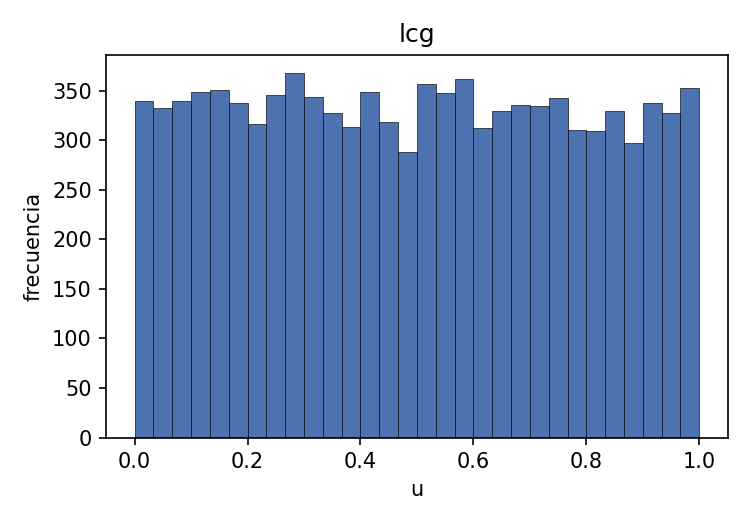
\includegraphics[width=0.6\textwidth]{figures/hist_lcg.png}
\caption{Histograma de 10{,}000 valores generados con el LCG, normalizados a $[0,1]$.}
\end{figure}

Con $N=10{,}000$ valores, la prueba chi-cuadrado de bondad de ajuste (20 categorías, 19 grados de libertad) dio un estadístico $\chi^2 = 28.39$ con $p = 0.076$: al ser mayor que $0.05$ no se rechaza la hipótesis de uniformidad. La autocorrelación de retardo 1 fue $r = 0.0022$ con $p = 0.824$, es decir, no hay evidencia de dependencia serial entre valores consecutivos.

\begin{figure}[H]
\centering
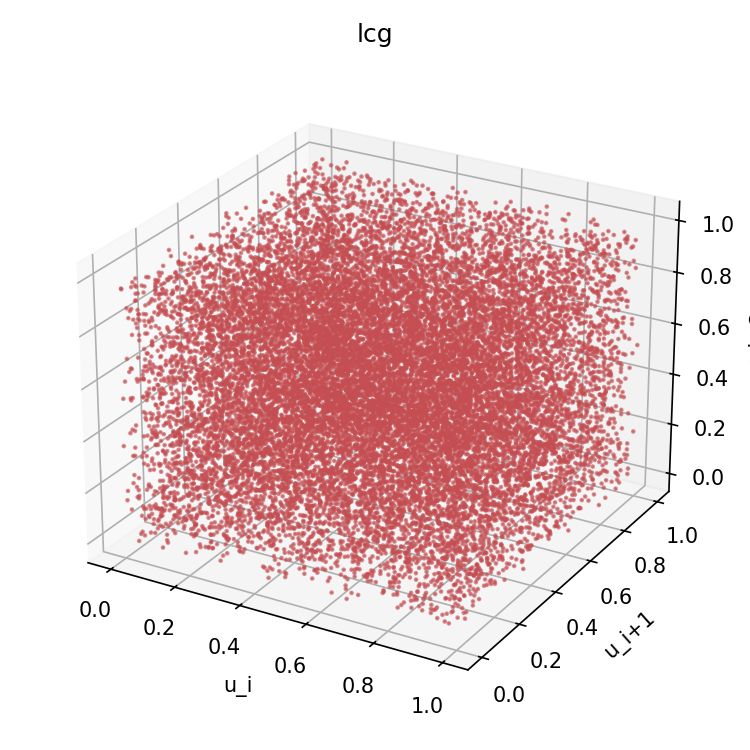
\includegraphics[width=0.55\textwidth]{figures/espectral_lcg.png}
\caption{Ternas consecutivas $(u_i, u_{i+1}, u_{i+2})$ del LCG en el cubo $[0,1]^3$.}
\end{figure}

Las ternas del LCG llenan el cubo de manera homogénea desde cualquier ángulo de observación, sin estructura visible. Esto es consistente con haber elegido parámetros que satisfacen Hull--Dobell: un buen LCG no debería mostrar ningún patrón geométrico en la prueba espectral.

\subsection{Método de cuadrados medios}

El método de cuadrados medios, propuesto por von Neumann, eleva al cuadrado la semilla actual y extrae los dígitos centrales como el siguiente término de la secuencia. Con $d$ dígitos por término, si $x_n$ tiene $d$ dígitos, $x_n^2$ tiene hasta $2d$ dígitos, y $x_{n+1}$ se forma tomando los $d$ dígitos centrales de ese cuadrado (rellenando con ceros a la izquierda si hace falta).

\begin{algorithm}[H]
\caption{Método de cuadrados medios}
\begin{algorithmic}[1]
\Require semilla $x_0$ de $d$ dígitos
\For{$n = 0, 1, 2, \dots$}
    \State $y \gets x_n^2$, escrito con $2d$ dígitos (rellenando con ceros a la izquierda)
    \State $x_{n+1} \gets$ los $d$ dígitos centrales de $y$
    \State $u_{n+1} \gets x_{n+1} / 10^d$
\EndFor
\end{algorithmic}
\end{algorithm}

No existe una fórmula cerrada para el período de este método: al ser un mapeo determinista sobre un conjunto finito de $10^d$ estados, eventualmente entra en un ciclo, pero ese ciclo suele ser mucho más corto que $10^d$, y en muchos casos degenera rápidamente a 0 o a ciclos muy cortos. Se usó $d=8$ dígitos y semilla $x_0 = 57282719$.

\begin{figure}[H]
\centering
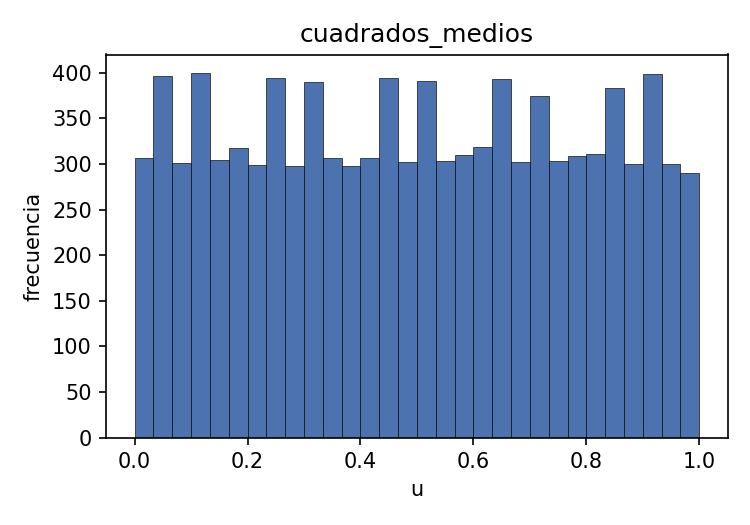
\includegraphics[width=0.6\textwidth]{figures/hist_cuadrados_medios.png}
\caption{Histograma de 10{,}000 valores generados con cuadrados medios.}
\end{figure}

A simple vista el histograma parece razonablemente uniforme, pero muestra un patrón de peine (barras alternadamente más altas y más bajas). La prueba chi-cuadrado lo confirma de forma contundente: $\chi^2 = 152.94$, $p \approx 0.0000$, rechazando uniformidad con un margen enorme. La autocorrelación de retardo 1 también resultó significativa ($r=-0.039$, $p=0.0001$). Esto es exactamente la falla clásica del método: la secuencia cae en ciclos cortos que repiten un subconjunto pequeño de valores muchas veces, lo que produce un histograma visualmente aceptable pero estadísticamente muy alejado de una uniforme real.

\subsection{Mersenne Twister}

El Mersenne Twister (variante MT19937) mantiene un estado interno de $n=624$ palabras de 32 bits. En cada bloque de $n$ salidas se aplica una recurrencia de "twist" sobre el estado, y cada palabra extraída pasa además por una transformación de temple (tempering) que mejora sus propiedades de equidistribución.

\begin{algorithm}[H]
\caption{Mersenne Twister (MT19937), esquema general}
\begin{algorithmic}[1]
\Require semilla $x_0$
\State Inicializar el arreglo de estado $mt[0..623]$ a partir de $x_0$ mediante un LCG auxiliar
\For{cada bloque de 624 salidas}
    \For{$i = 0, \dots, 623$}
        \State $y \gets (mt[i]\ \&\ \texttt{0x80000000}) + (mt[(i+1)\bmod 624]\ \&\ \texttt{0x7fffffff})$
        \State $mt[i] \gets mt[(i+397)\bmod 624] \oplus (y \gg 1)$
        \If{$y$ es impar}
            \State $mt[i] \gets mt[i] \oplus \texttt{0x9908b0df}$
        \EndIf
    \EndFor
\EndFor
\State $y \gets mt[i]$
\State $y \gets y \oplus (y \gg 11)$
\State $y \gets y \oplus ((y \ll 7)\ \&\ \texttt{0x9d2c5680})$
\State $y \gets y \oplus ((y \ll 15)\ \&\ \texttt{0xefc60000})$
\State $y \gets y \oplus (y \gg 18)$
\State \Return $y / 2^{32}$
\end{algorithmic}
\end{algorithm}

El período del Mersenne Twister es $2^{19937}-1$, y su nombre viene precisamente de que ese número es un primo de Mersenne. La implementación se validó comparando la primera salida cruda con semilla $5489$ contra el valor de referencia publicado, $3499211612$, que coincidió exactamente.

\begin{figure}[H]
\centering
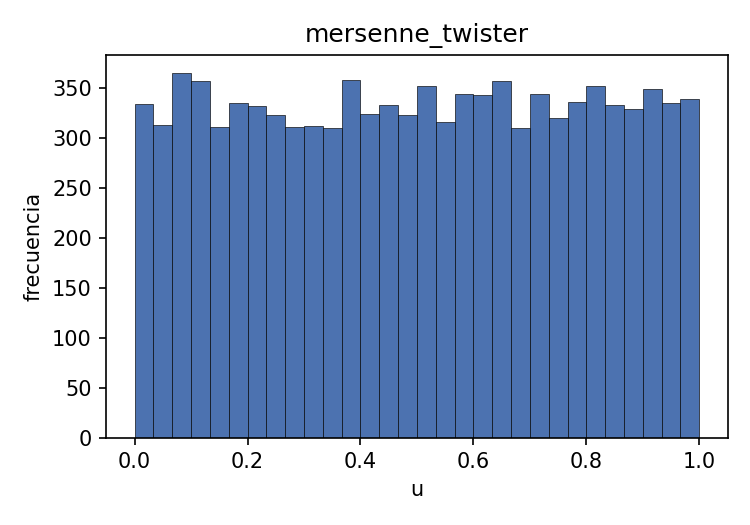
\includegraphics[width=0.6\textwidth]{figures/hist_mersenne_twister.png}
\caption{Histograma de 10{,}000 valores generados con Mersenne Twister.}
\end{figure}

Con semilla $5489$ se obtuvo $\chi^2 = 12.14$, $p=0.880$ para uniformidad, y $r=-0.0026$, $p=0.797$ para independencia serial: ambas pruebas son plenamente consistentes con una secuencia uniforme e independiente.

\subsection{Blum Blum Shub}

Blum Blum Shub genera bits (o números) mediante $x_{n+1} = x_n^2 \bmod M$, donde $M = pq$ es producto de dos primos grandes, ambos congruentes con $3 \bmod 4$ (un entero de Blum). Su seguridad depende de la dificultad de calcular residuos cuadráticos módulo $M$ sin conocer su factorización, un problema tan difícil como factorizar $M$.

\begin{algorithm}[H]
\caption{Blum Blum Shub}
\begin{algorithmic}[1]
\Require semilla $x_0$ coprima con $M=pq$, $p\equiv q\equiv 3 \pmod 4$
\For{$n = 0, 1, 2, \dots$}
    \State $x_{n+1} \gets x_n^2 \bmod M$
    \State $u_{n+1} \gets x_{n+1} / M$
\EndFor
\end{algorithmic}
\end{algorithm}

Para esta tarea se usaron los primos $p=300007$ y $q=300163$ (ambos $\equiv 3 \bmod 4$), con $M = 90{,}051{,}001{,}141$ y semilla $x_0=987654323$. Estos primos son mucho más pequeños que los que se usarían en una aplicación criptográfica real (donde $p$ y $q$ tendrían cientos de dígitos); se eligieron de este tamaño únicamente para que generar miles de valores fuera rápido en Python puro.

\begin{figure}[H]
\centering
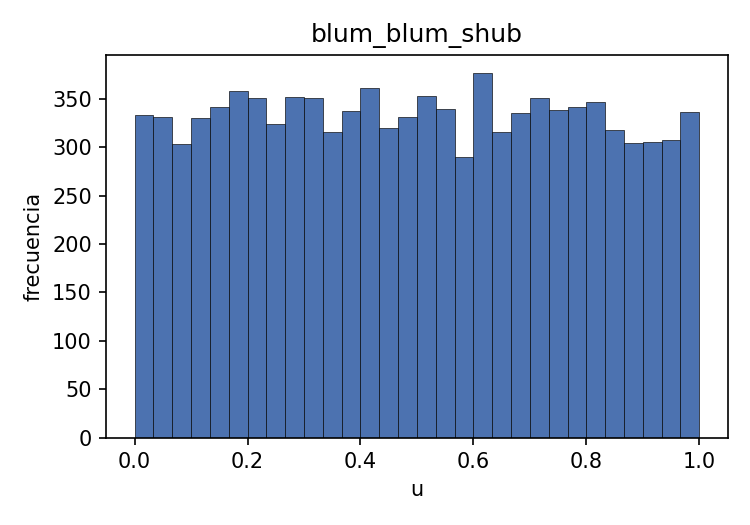
\includegraphics[width=0.6\textwidth]{figures/hist_blum_blum_shub.png}
\caption{Histograma de 10{,}000 valores generados con Blum Blum Shub.}
\end{figure}

Se obtuvo $\chi^2=29.66$, $p=0.056$ para uniformidad (justo por encima del umbral usual de 0.05) y $r=0.0174$, $p=0.083$ para independencia serial: no hay evidencia fuerte de desviación de la uniformidad ni de dependencia serial, aunque el $p$-valor de uniformidad queda cerca del límite.

\subsection{RANDU}
\label{sec:randu-generador}

RANDU es un caso particular de LCG con $a=65539=2^{16}+3$, $c=0$ y $m=2^{31}$, usado en las computadoras IBM System/360 durante los años sesenta. Es históricamente célebre por lo mal elegido de su multiplicador.

\begin{algorithm}[H]
\caption{RANDU}
\begin{algorithmic}[1]
\Require semilla impar $x_0$
\For{$n = 0, 1, 2, \dots$}
    \State $x_{n+1} \gets (65539 \cdot x_n) \bmod 2^{31}$
    \State $u_{n+1} \gets x_{n+1} / 2^{31}$
\EndFor
\end{algorithmic}
\end{algorithm}

Debido a que $m=2^{31}$ y $a-1 = 65538$ no cumple la condición de Hull--Dobell relacionada con los factores de $m$, el período efectivo de RANDU con semilla impar es $2^{29}$, es decir, un cuarto del máximo teórico $m$. La semilla usada fue $x_0=1$.

\begin{figure}[H]
\centering
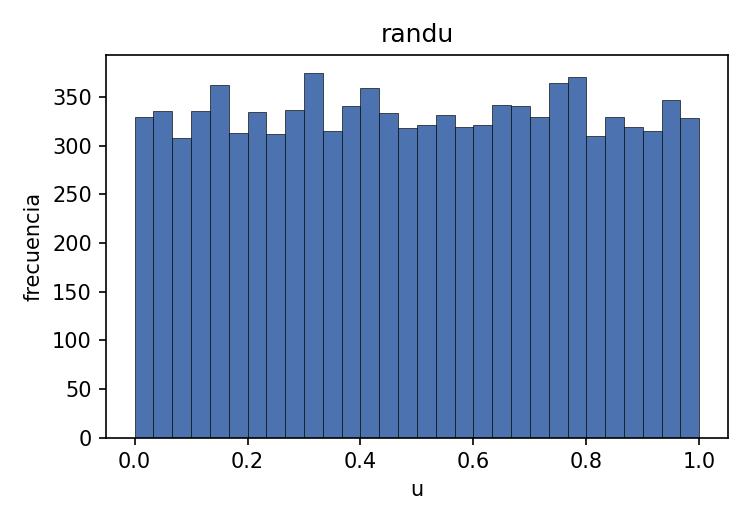
\includegraphics[width=0.6\textwidth]{figures/hist_randu.png}
\caption{Histograma de 10{,}000 valores generados con RANDU.}
\end{figure}

En una dimensión, RANDU pasa las pruebas sin problema: $\chi^2=15.16$, $p=0.712$ para uniformidad, y $r=0.0133$, $p=0.184$ para independencia serial. Esto ya es una lección importante: las pruebas de uniformidad e independencia serial de retardo 1 son \emph{incapaces} de detectar el defecto real de RANDU, que solo aparece al observar ternas de valores consecutivos.

\begin{figure}[H]
\centering
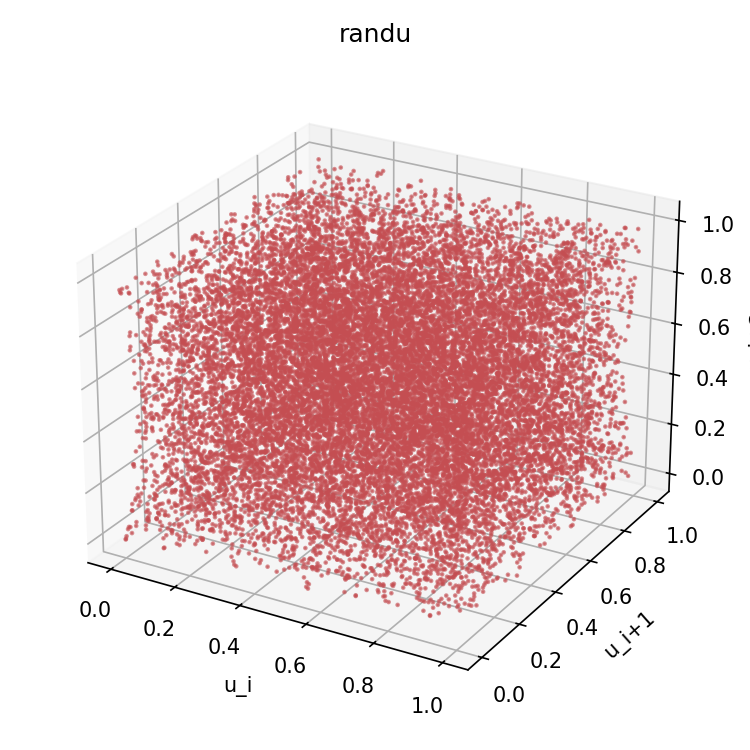
\includegraphics[width=0.48\textwidth]{figures/espectral_randu.png}
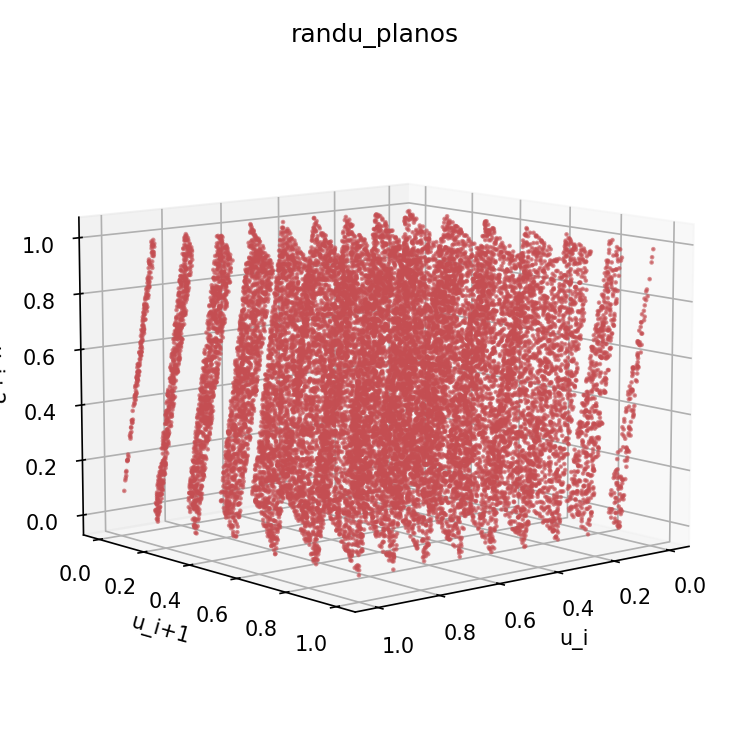
\includegraphics[width=0.48\textwidth]{figures/espectral_randu_planos.png}
\caption{Ternas consecutivas de RANDU en $[0,1]^3$. Izquierda: ángulo de vista genérico, donde el defecto no es evidente. Derecha: mismo conjunto de puntos visto desde el ángulo que deja ver de canto los hiperplanos sobre los que caen todas las ternas.}
\end{figure}

Puede demostrarse que toda terna consecutiva de RANDU satisface exactamente $x_{n+2} = 6x_{n+1} - 9x_n \pmod{2^{31}}$, lo cual implica que los puntos $(u_n, u_{n+1}, u_{n+2})$ caen sobre la familia de planos paralelos $9u_n - 6u_{n+1} + u_{n+2} = k$ para $k$ entero. Dentro del cubo $[0,1]^3$ esa expresión solo puede tomar unos 15 valores enteros distintos, así que las ternas de RANDU quedan confinadas a apenas 15 hiperplanos, en vez de llenar el cubo. Desde un ángulo de vista genérico esto no salta a la vista, pero basta rotar la cámara para verlo con total claridad. Esta es la falla que Marsaglia documentó en \emph{Random Numbers Fall Mainly in the Planes}.

\subsection{Comparación de velocidad, período, seguridad y casos de uso}

\begin{table}[H]
\centering
\small
\begin{tabularx}{\textwidth}{l X X c X}
\toprule
Algoritmo & Velocidad (núm/s) & Período & Seguro & Uso típico \\
\midrule
LCG & $\sim 1.05\times 10^{7}$ & $2^{32}$ (buenos parámetros) & No & Simulaciones, videojuegos \\
Cuadrados medios & $\sim 4.4\times 10^{6}$ & Corto e impredecible & No & Interés histórico/didáctico \\
Mersenne Twister & $\sim 1.9\times 10^{6}$ & $2^{19937}-1$ & No & Simulación científica, \texttt{random} \\
Blum Blum Shub & $\sim 1.0\times 10^{7 \ *}$ & Grande si $p,q$ son primos seguros & Sí (criptográfico) & Claves, cifrado de flujo \\
RANDU & $\sim 1.2\times 10^{7}$ & $2^{29}$ (defectuoso) & No & Ninguno (obsoleto) \\
\bottomrule
\end{tabularx}
\caption{Comparación de los cinco algoritmos. Las velocidades se midieron generando 100{,}000 números en la misma máquina. ($^*$) La velocidad de Blum Blum Shub depende fuertemente del tamaño de los primos: aquí se usaron primos pequeños por rapidez, no primos criptográficamente seguros.}
\end{table}

Mersenne Twister resulta más lento que LCG y RANDU porque cada salida involucra varias operaciones de temple además de la recurrencia de estado, mientras que LCG y RANDU son una sola multiplicación y suma módulo $m$. Blum Blum Shub, pese a ser el único diseñado con garantías criptográficas, aquí resulta rápido solo porque se usaron primos de unas pocas decenas de bits; con primos de tamaño criptográfico real ($2048$ bits o más) sería órdenes de magnitud más lento que los demás, ya que ese costo computacional es precisamente lo que sostiene su seguridad.

\subsection{Comparación con las librerías estándar de Python}

Se comparó la implementación propia de Mersenne Twister contra \texttt{random.Random} (que también usa MT19937 internamente, implementado en C) y contra \texttt{secrets.SystemRandom} (que obtiene aleatoriedad del sistema operativo, pensado para uso criptográfico). Se generaron $300{,}000$ números con cada uno:

\begin{table}[H]
\centering
\begin{tabular}{lccc}
\toprule
Generador & Tiempo (s) & $\chi^2$ & $p$-valor \\
\midrule
Mersenne Twister propio & 0.157 & 21.93 & 0.288 \\
\texttt{random} estándar & 0.010 & 26.14 & 0.126 \\
\texttt{secrets} (CSPRNG) & 0.193 & 33.59 & 0.021 \\
\bottomrule
\end{tabular}
\caption{Comparación de velocidad y bondad de ajuste, $N=300{,}000$.}
\end{table}

La versión de \texttt{random} de la librería estándar es unas 15 veces más rápida que la implementación propia porque su ciclo interno está escrito en C, mientras que la nuestra corre en Python puro instrucción por instrucción. \texttt{secrets} resulta el más lento de los tres, un costo esperado: para ser criptográficamente seguro no puede depender de un estado interno predecible como el de un Mersenne Twister, así que consulta al sistema operativo en cada llamada. El $p$-valor bajo de \texttt{secrets} en esta corrida particular no indica ningún defecto real, es simplemente la variabilidad normal de una prueba de hipótesis: repitiendo el experimento con otra semilla del sistema el resultado cambia.

\section{Fundamento de Monte Carlo: el estimador y su error}

\subsection{Insesgadez del estimador}

\begin{figure}[H]
\centering
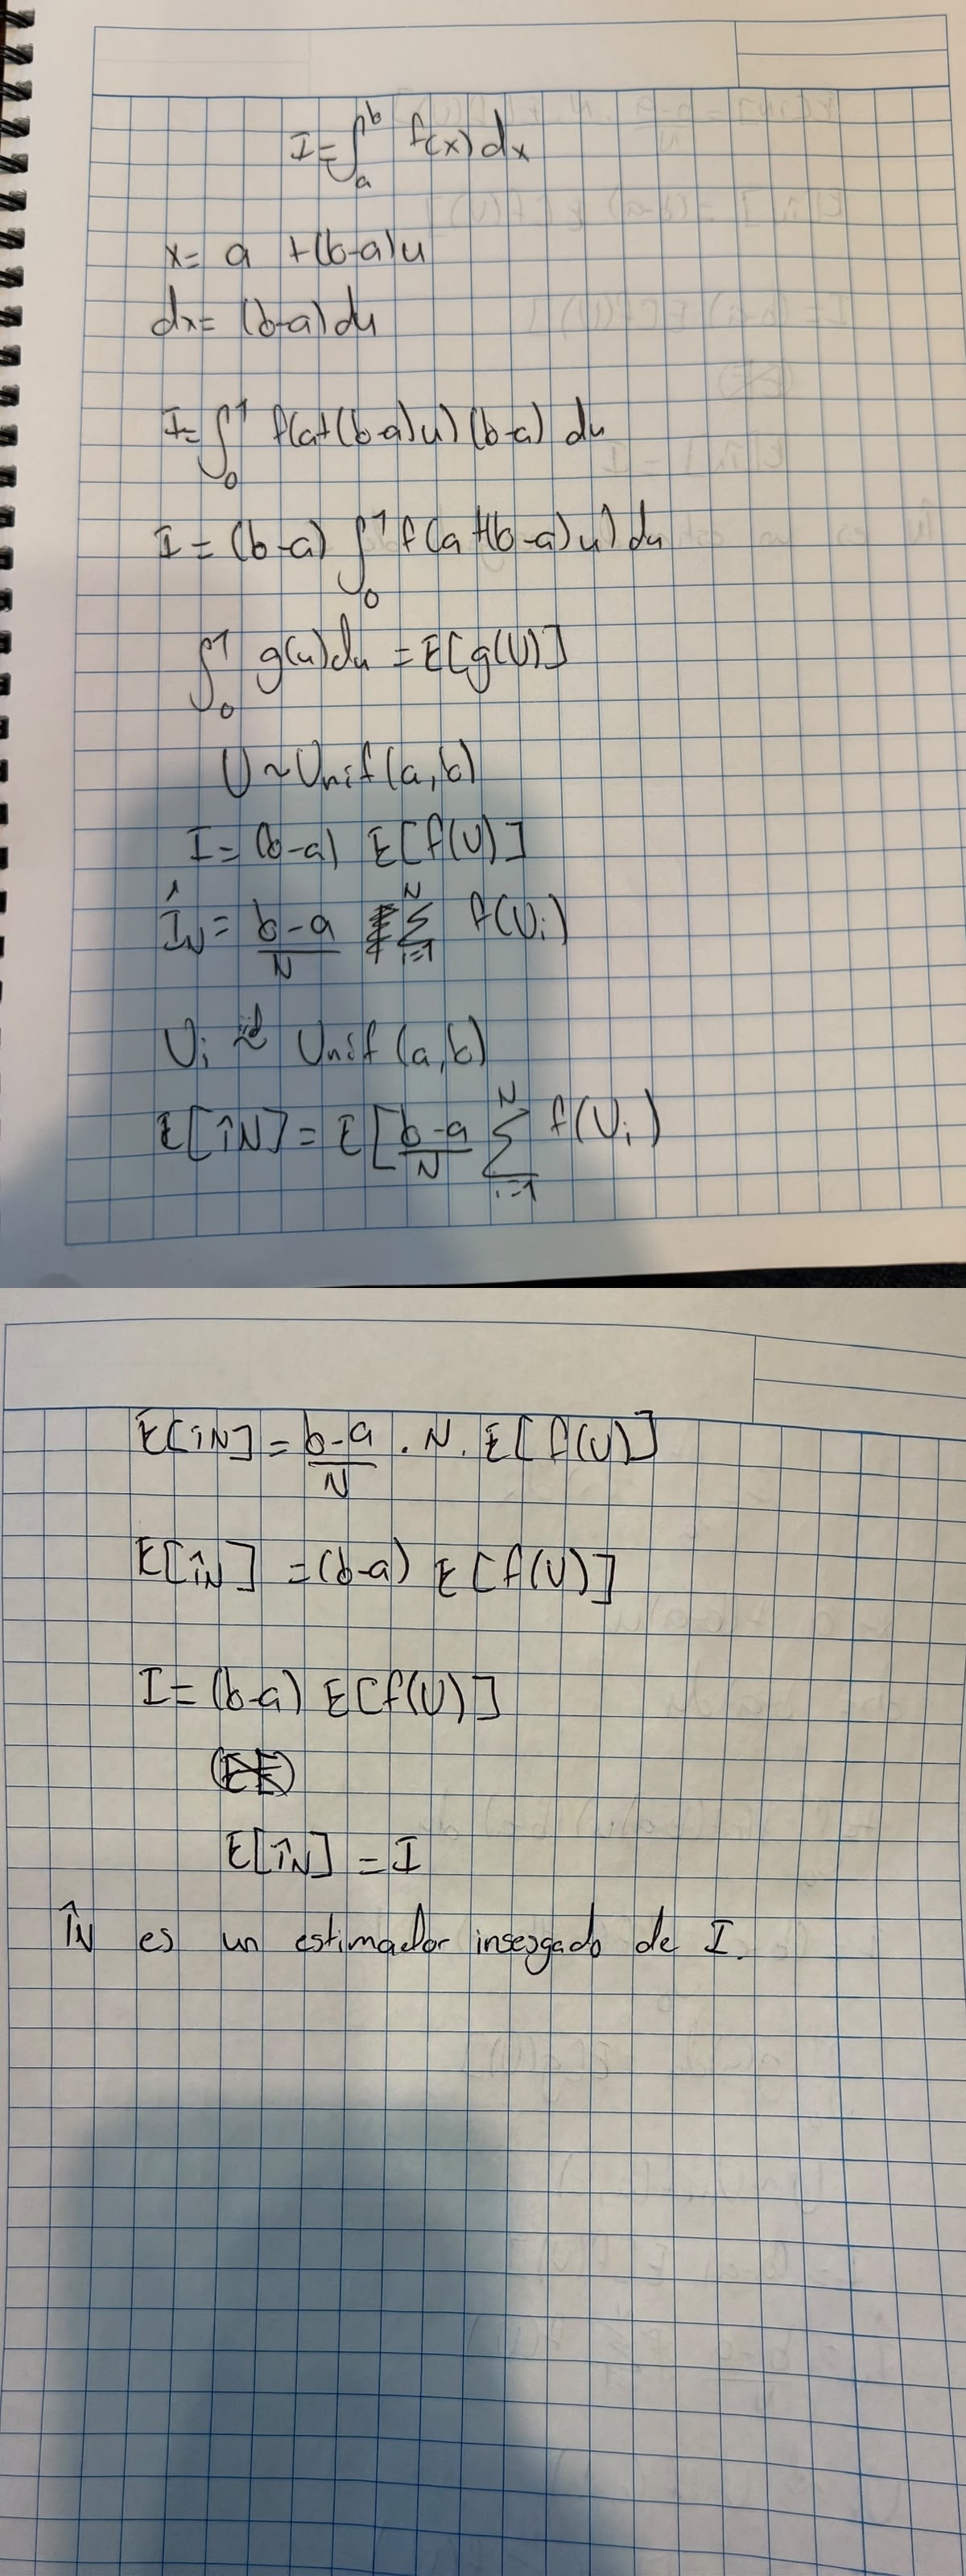
\includegraphics[width=0.85\textwidth,height=0.8\textheight,keepaspectratio]{figures/derivaciones/insesgadez.jpg}
\caption{Derivación a mano de $I=(b-a)\mathbb{E}[f(U)]$ y de $\mathbb{E}[\hat I_N]=I$.}
\end{figure}

\subsection{Varianza del estimador y tasa de convergencia}
\label{sec:varianza}

\begin{figure}[H]
\centering
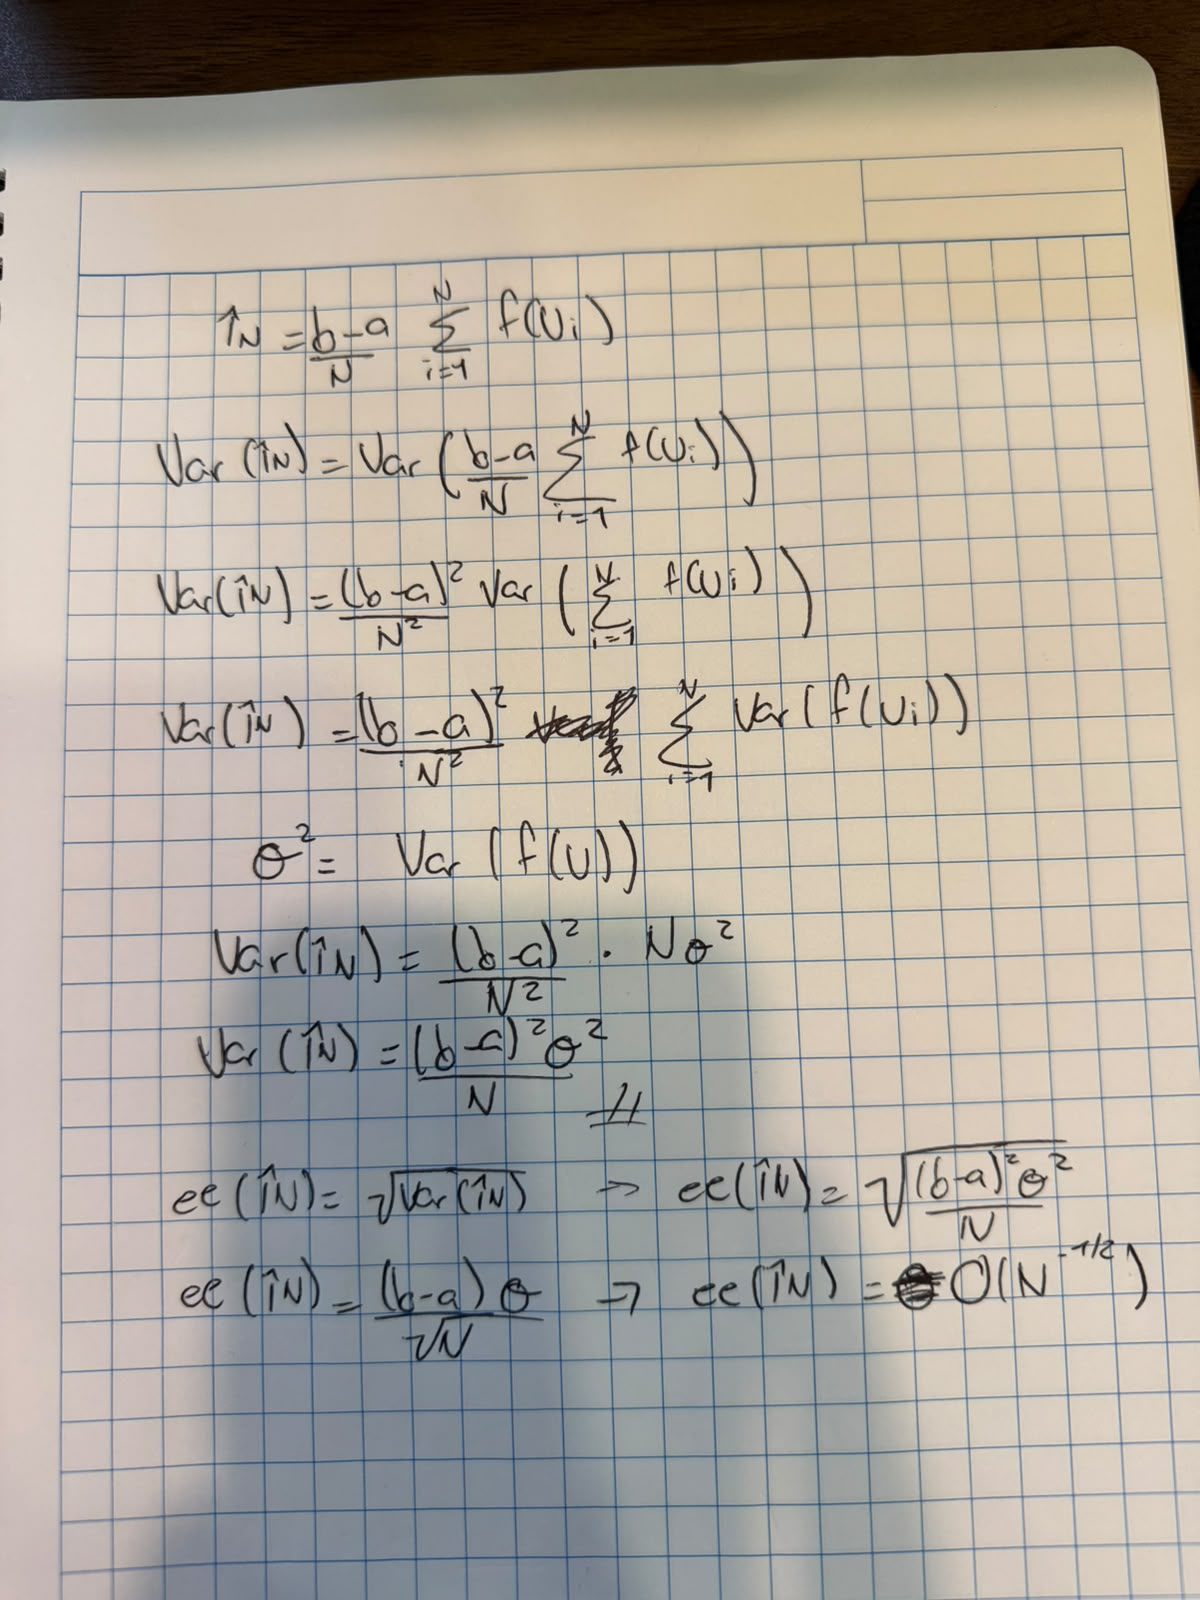
\includegraphics[width=0.85\textwidth,height=0.8\textheight,keepaspectratio]{figures/derivaciones/varianza.jpg}
\caption{Derivación a mano de $\mathrm{Var}(\hat I_N)$ y de por qué el error estándar decae como $O(N^{-1/2})$.}
\end{figure}

Esta tasa no depende de la dimensión del problema porque la Ley de los Grandes Números y el Teorema del Límite Central se aplican sobre el promedio de variables aleatorias escalares $f(U_i)$, sin importar de qué espacio provienen los $U_i$: lo único que entra en la varianza del estimador es $\mathrm{Var}(f(U))$, un solo número real, nunca la dimensión de $U$. Un integrando en $d=20$ dimensiones tiene exactamente la misma tasa $O(N^{-1/2})$ que uno en $d=1$; lo que cambia con $d$ es qué tan grande es esa varianza, no la forma en que decae con $N$. Esta observación es la que hace útil a Monte Carlo en la Sección \ref{sec:altadim}: los métodos de cuadratura determinística sí empeoran con la dimensión, Monte Carlo no.

\subsection{Intervalo de confianza del 95\%}
\label{sec:ic}

\begin{figure}[H]
\centering
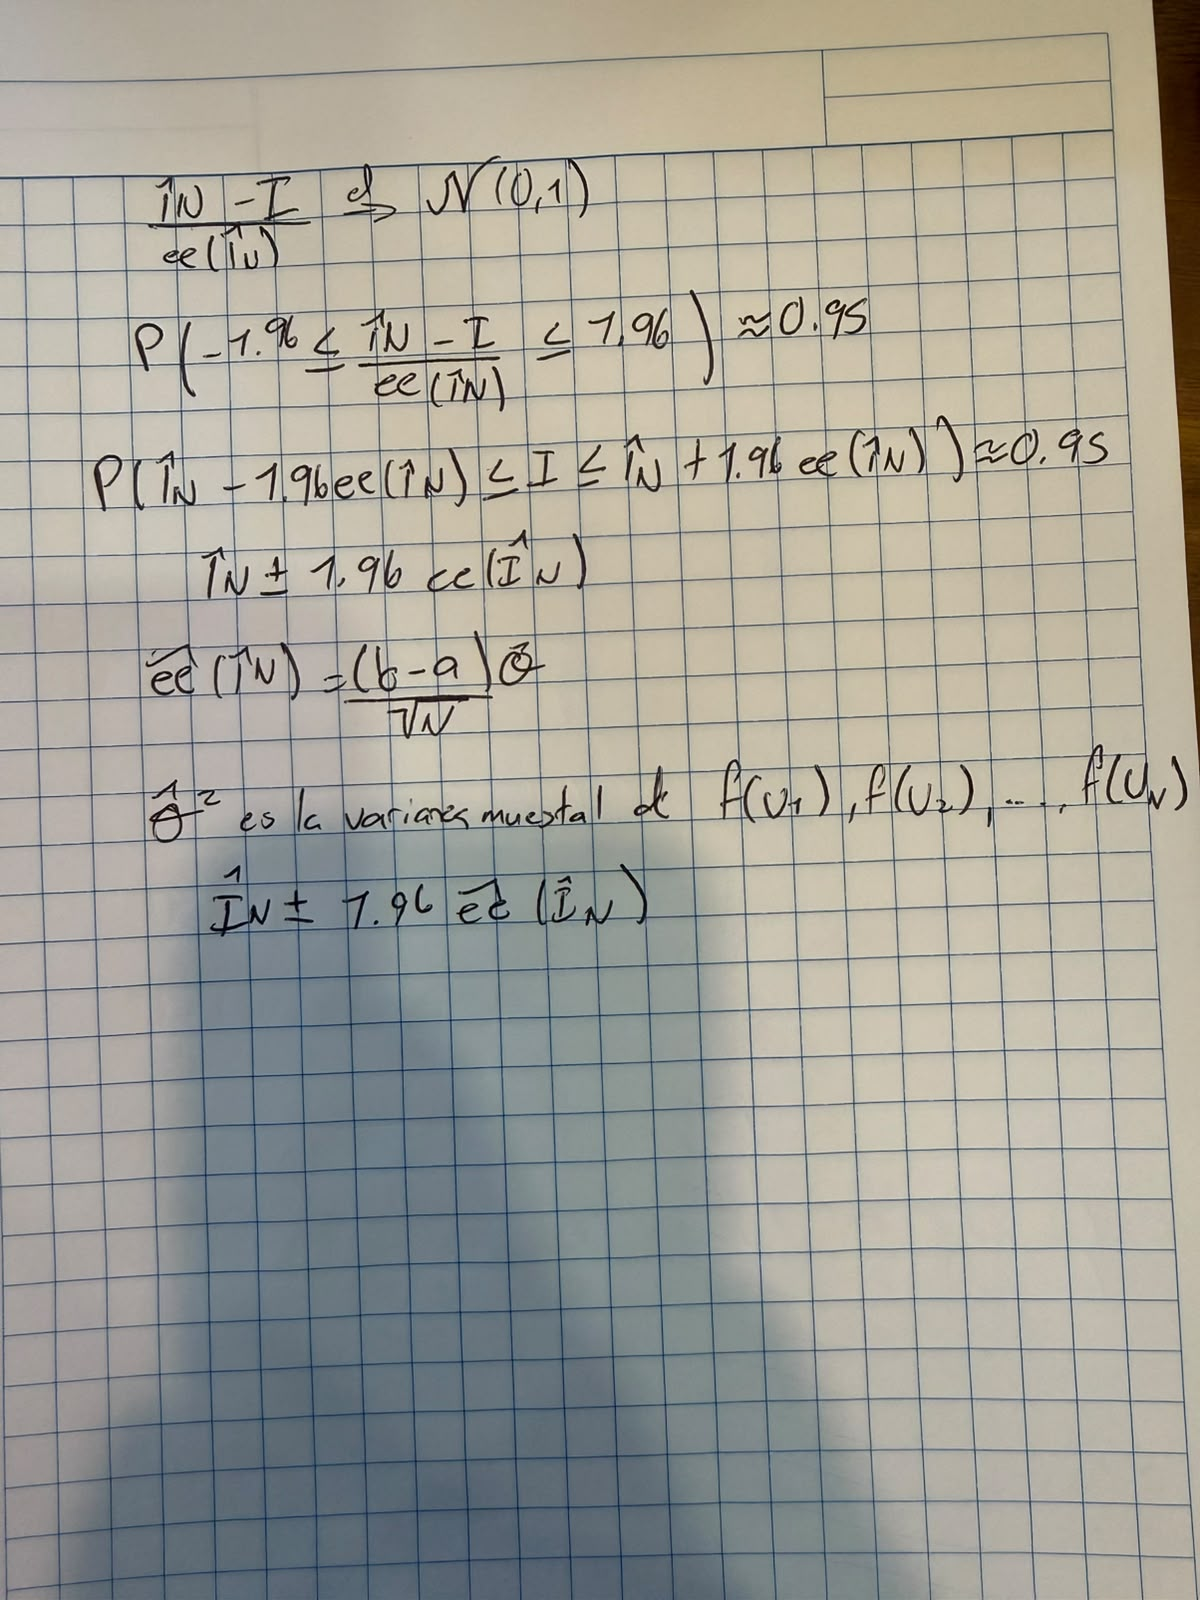
\includegraphics[width=0.85\textwidth,height=0.8\textheight,keepaspectratio]{figures/derivaciones/intervalo.jpg}
\caption{Construcción del intervalo de confianza del 95\% para $\hat I_N$ usando el TLC.}
\end{figure}

De aquí en adelante todo estimador Monte Carlo reportado en este documento viene acompañado de su intervalo de confianza del 95\%, calculado como $\hat I_N \pm 1.96 \cdot \widehat{\mathrm{ee}}(\hat I_N)$, con $\widehat{\mathrm{ee}}(\hat I_N)$ el error estándar estimado a partir de la muestra.

\section{Calentamiento: integrales en una dimensión}
\label{sec:integrales1d}

Se implementó el estimador de la sección anterior en \texttt{src/montecarlo/estimator.py} y se aplicó a las dos integrales del enunciado, muestreando $U\sim\mathrm{Unif}(a,b)$ con la semilla $20250922$.

\subsection{Integral (a): $\int_0^1 \sin(\pi x)\,dx$}

El valor real es $2/\pi \approx 0.636620$. Con $N=1{,}000{,}000$ se obtuvo $\hat I_N = 0.636421$, con intervalo de confianza del 95\% $(0.635817,\ 0.637024)$, que en efecto contiene el valor real. El error absoluto fue de apenas $0.000199$.

\begin{figure}[H]
\centering
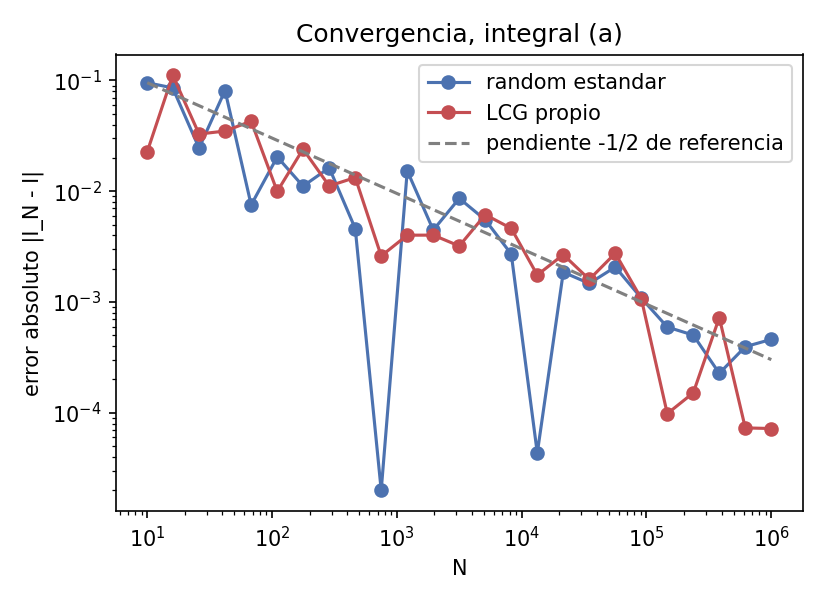
\includegraphics[width=0.6\textwidth]{figures/convergencia_a.png}
\caption{Error absoluto $|\hat I_N - I|$ contra $N$ en escala log-log, integral (a).}
\end{figure}

El ajuste de una recta a $\log_{10}|\hat I_N - I|$ contra $\log_{10} N$ dio una pendiente de $-0.454$, cercana a la tasa teórica $-1/2$ derivada en la Sección anterior. La diferencia con $-0.5$ exacto es simplemente ruido de una sola trayectoria: el error absoluto de una corrida particular no decae monótonamente, oscila alrededor de la tendencia $O(N^{-1/2})$, y una pendiente ajustada sobre una sola realización rara vez da exactamente $-0.5$.

\subsection{Integral (b): $\int_0^2 \frac{1}{\sqrt{2\pi}} e^{-x^2/2}\,dx$}

El valor real es $\Phi(2)-\Phi(0) \approx 0.477250$. Con $N=1{,}000{,}000$ se obtuvo $\hat I_N = 0.477237$, IC 95\% $(0.476786,\ 0.477689)$, error absoluto $0.000013$.

\begin{figure}[H]
\centering
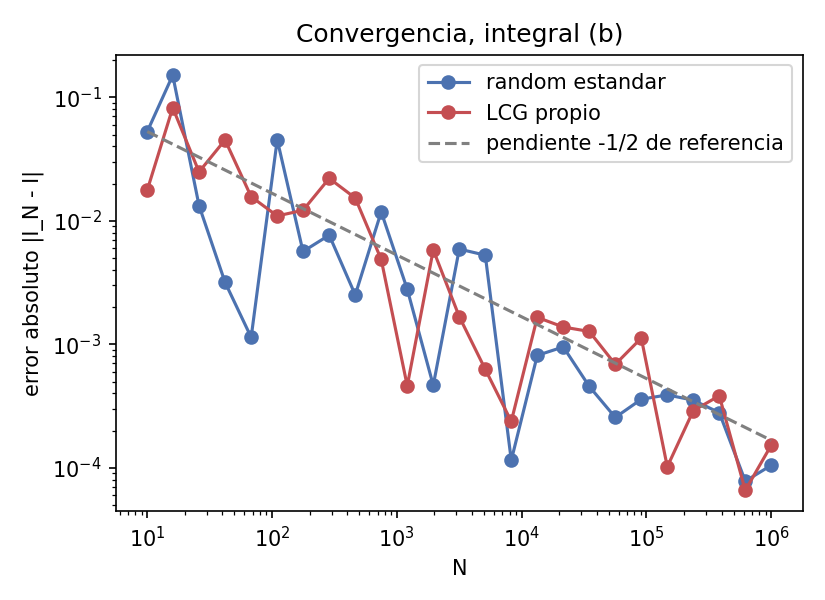
\includegraphics[width=0.6\textwidth]{figures/convergencia_b.png}
\caption{Error absoluto $|\hat I_N - I|$ contra $N$ en escala log-log, integral (b).}
\end{figure}

Aquí la pendiente ajustada fue $-0.493$, todavía más cercana a $-1/2$. Ambos casos confirman empíricamente la tasa de convergencia derivada analíticamente.

\subsection{Comparación entre generadores}

Las dos figuras anteriores incluyen, además del generador \texttt{random} estándar de Python, la misma integral estimada con el LCG propio de la Parte 1 (Sección 1.1), usando en cada punto $N$ un bloque nuevo de valores de esa misma secuencia. Las dos curvas de error son estadísticamente indistinguibles entre sí y ambas siguen la tendencia $O(N^{-1/2})$: para una integral de buen comportamiento en una dimensión, un LCG con parámetros razonables rinde tan bien como el generador de la librería estándar. La diferencia entre generadores solo se vuelve relevante cuando el generador tiene defectos estructurales serios, como se ve con RANDU en la Sección \ref{sec:randu}.

\section{Alta dimensión y la maldición de la dimensionalidad}
\label{sec:altadim}

Se implementó un estimador Monte Carlo para el volumen de la bola unitaria $V_d$ en $d$ dimensiones, muestreando puntos uniformes en el cubo $[-1,1]^d$ con el LCG propio y contando la fracción que cae dentro de la bola. Como referencia se usó el valor cerrado $V_d = \pi^{d/2}/\Gamma(d/2+1)$, y como contraparte determinística se implementó una cuadratura por rejilla, evaluando el indicador en el centro de cada celda de una malla de $m$ subdivisiones por eje, con $m=\lfloor N^{1/d}\rfloor$ para igualar aproximadamente el presupuesto de puntos $N=1{,}000{,}000$ entre ambos métodos.

\begin{table}[H]
\centering
\begin{tabular}{lccc}
\toprule
$d$ & $V_d$ real & Estimado MC (IC 95\%) & Error absoluto MC \\
\midrule
2 & 3.14159 & 3.14244 $\ (3.13922,\ 3.14566)$ & 0.000847 \\
5 & 5.26379 & 5.26288 $\ (5.23963,\ 5.28613)$ & 0.000909 \\
10 & 2.55016 & 2.46374 $\ (2.36542,\ 2.56207)$ & 0.086420 \\
20 & 0.025807 & 0.000000 $\ (0,\ 3.14573)$ & 0.025807 \\
\bottomrule
\end{tabular}
\caption{Estimación Monte Carlo de $V_d$ con $N=1{,}000{,}000$ puntos, semilla base $20250923$.}
\end{table}

En $d=20$ no se registró ni un solo acierto: de los $10^6$ puntos muestreados, se esperaban en promedio $N \cdot V_{20}/2^{20} \approx 1{,}000{,}000 \times 2.46\times 10^{-8} \approx 0.025$ aciertos, así que obtener cero es exactamente lo esperado, no una falla del código. Con cero aciertos el intervalo de confianza normal de la Sección \ref{sec:ic} degenera (varianza estimada cero), así que se reporta en su lugar una cota superior aproximada con la regla de tres, $3/N$, escalada por $2^d$.

\subsection{Comparación contra cuadratura determinística}

\begin{table}[H]
\centering
\begin{tabular}{lcccc}
\toprule
$d$ & $m$ (rejilla) & Puntos rejilla & Estimado rejilla & Error absoluto rejilla \\
\midrule
2 & 1000 & 1{,}000{,}000 & 3.14182 & 0.000231 \\
5 & 16 & 1{,}048{,}576 & 5.31152 & 0.047734 \\
10 & 4 & 1{,}048{,}576 & 1.00000 & 1.550160 \\
20 & 2 & 1{,}048{,}576 & 0.00000 & 0.025807 \\
\bottomrule
\end{tabular}
\caption{Cuadratura por rejilla con presupuesto de puntos comparable al de Monte Carlo.}
\end{table}

Con un presupuesto de puntos similar, la rejilla le gana a Monte Carlo en $d=2$ (su error es casi 4 veces menor), pero para $d=5$ ya es Monte Carlo el que gana claramente, y para $d=10$ la rejilla es catastrófica: con solo $m=4$ subdivisiones por eje, la malla es tan gruesa que ni siquiera logra resolver la curvatura de la esfera y termina estimando el volumen de un solo cubito central, muy lejos del valor real. En $d=20$ ambos métodos fallan por completo con este presupuesto, pero por razones distintas: la rejilla porque $m=2$ es una resolución absurda para captar una esfera, y Monte Carlo porque la probabilidad de acierto es demasiado baja para el número de muestras disponible.

\begin{table}[H]
\centering
\begin{tabular}{lc}
\toprule
$d$ & Puntos necesarios en rejilla ($m=10$) \\
\midrule
2 & 100 \\
5 & 100{,}000 \\
10 & 10{,}000{,}000{,}000 \\
20 & 100{,}000{,}000{,}000{,}000{,}000{,}000 \\
\bottomrule
\end{tabular}
\caption{Número de puntos $m^d$ que necesitaría la rejilla para mantener 10 subdivisiones por eje.}
\end{table}

El número de puntos de la rejilla crece como $m^d$: exponencial en la dimensión. Mantener una resolución fija de 10 subdivisiones por eje es factible en $d=2$ (cien puntos) pero ya es completamente inalcanzable en $d=20$ ($10^{20}$ puntos, más que cualquier cómputo razonable podrá evaluar jamás). Esta es la esencia de la maldición de la dimensionalidad: los métodos que discretizan cada eje por separado sufren un costo que se multiplica, no se suma, con cada dimensión nueva. Monte Carlo, en cambio, mantiene su tasa de error $O(N^{-1/2})$ sin importar $d$ (Sección \ref{sec:varianza}), lo que explica por qué termina siendo la única opción viable en dimensiones altas, aun cuando su desempeño relativo en $d=2$ sea mediocre frente a una rejilla fina.

\subsection{Por qué el muestreo uniforme se vuelve ineficiente}

\begin{figure}[H]
\centering
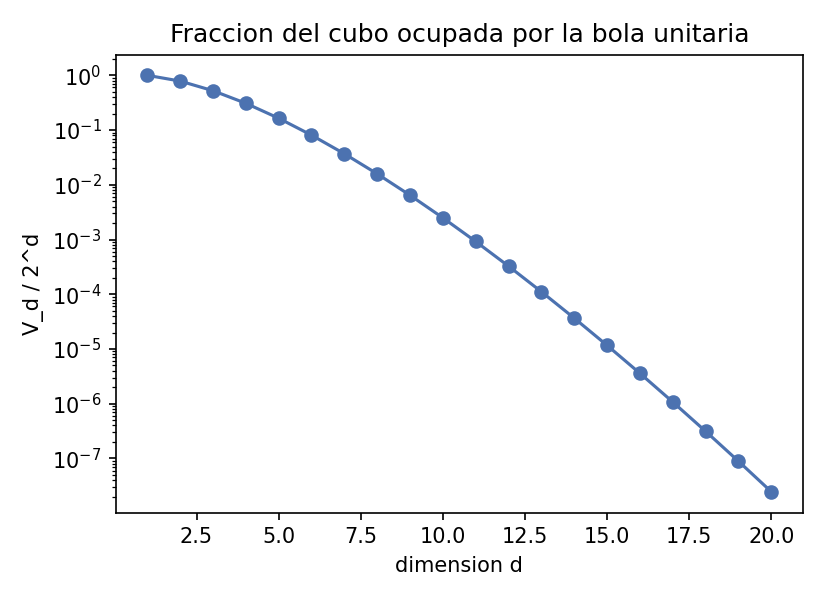
\includegraphics[width=0.6\textwidth]{figures/fraccion_volumen.png}
\caption{Fracción del volumen del cubo $[-1,1]^d$ ocupada por la bola unitaria, $V_d/2^d$, en escala logarítmica.}
\end{figure}

La fracción $V_d/2^d$ decae exponencialmente con $d$: en $d=2$ la bola todavía ocupa un 79\% del cuadrado, pero en $d=20$ ocupa apenas $2.46\times 10^{-8}$ del cubo. Esto revela que, en alta dimensión, casi todo el volumen de un hipercubo vive cerca de sus esquinas y muy lejos del centro: la masa se concentra en las "puntas" del cubo, una manifestación geométrica directa de la maldición de la dimensionalidad. Para un estimador Monte Carlo esto es letal si se muestrea ingenuamente en el cubo entero, porque la enorme mayoría de los puntos generados caen en la región irrelevante (fuera de la bola) y aportan cero información sobre la cantidad que se quiere medir; se necesitan cantidades astronómicas de muestras para obtener siquiera unos pocos aciertos útiles. Esta es precisamente la motivación detrás de las técnicas de reducción de varianza y de muestreo por importancia: en vez de muestrear a ciegas donde casi nunca hay señal, conviene concentrar el muestreo donde el integrando realmente aporta.

\section{Reducción de varianza}

El error de Monte Carlo decae como $\sigma/\sqrt N$, así que además de aumentar $N$ la única otra vía es reducir $\sigma$. Se implementaron y compararon dos técnicas, variables antitéticas y variables de control, aplicadas a las integrales de la Sección \ref{sec:integrales1d}, usando en todos los casos $N=2{,}000{,}000$ muestras uniformes con semilla $20250924$.

\subsection{Variables antitéticas}

La idea es reemplazar cada muestra $U_i$ por el promedio $Y_i = \tfrac{1}{2}\big(f(U_i) + f(a+b-U_i)\big)$: si $f(U)$ y $f(a+b-U)$ están negativamente correlacionadas, promediarlas reduce la varianza. Comparando a igualdad de número total de evaluaciones de $f$ ($N$ evaluaciones simples contra $N/2$ pares), el factor de reducción de varianza es $\mathrm{Var}(f(U)) / \big(2\,\mathrm{Var}(Y)\big)$.

Para la integral (a), $f(x)=\sin(\pi x)$ en $[0,1]$, el par antitético es $x$ y $1-x$, y como $\sin(\pi(1-x)) = \sin(\pi x)$ exactamente, ambos miembros del par valen siempre lo mismo: $Y_i = f(U_i)$ sin ninguna reducción de varianza, solo el doble de costo. El experimento lo confirma: $\mathrm{Var}(f(U)) = 0.094657$ y $\mathrm{Var}(Y) = 0.094657$ (idénticas), dando un factor de reducción de $0.5$, es decir, antitéticas resulta \emph{el doble de caro} que Monte Carlo simple para la misma precisión en este caso.

Para la integral (b), $f$ es la densidad normal estándar en $[0,2]$, monótona decreciente en ese intervalo. Aquí el par antitético $x, 2-x$ sí está negativamente correlacionado: $\mathrm{Var}(f(U))=0.013253$ contra $\mathrm{Var}(Y)=0.0000182$, dando un factor de reducción de $363$, equivalente a necesitar 363 veces menos muestras para el mismo error con Monte Carlo simple.

\subsection{Variables de control}

La idea es restar de $f(U)$ un múltiplo de una variable $g(U)$ de media conocida $\mu_g$: el estimador controlado $H = f(U) - c(g(U)-\mu_g)$ sigue siendo insesgado para cualquier $c$, y con $c^* = \mathrm{Cov}(f,g)/\mathrm{Var}(g)$ se minimiza $\mathrm{Var}(H) = \mathrm{Var}(f) - \mathrm{Cov}(f,g)^2/\mathrm{Var}(g)$. Se probaron dos controles para la integral (a):

\begin{itemize}
\item $g(x)=x$, con $\mu_g=0.5$: la correlación muestral con $\sin(\pi x)$ resultó $-0.0002$, esencialmente cero (tiene sentido: $\sin(\pi x)$ es simétrico alrededor de $x=0.5$ mientras que $x$ es una función lineal creciente, así que no hay relación lineal entre ambas). El factor de reducción fue $1.0000$: este control no ayuda en absoluto.
\item $g(x)=x(1-x)$, con $\mu_g=1/6$: esta función también es una joroba simétrica que se anula en los extremos, con una forma mucho más parecida a $\sin(\pi x)$. La correlación muestral resultó $0.9984$, casi perfecta, y el factor de reducción fue $318$.
\end{itemize}

\begin{figure}[H]
\centering
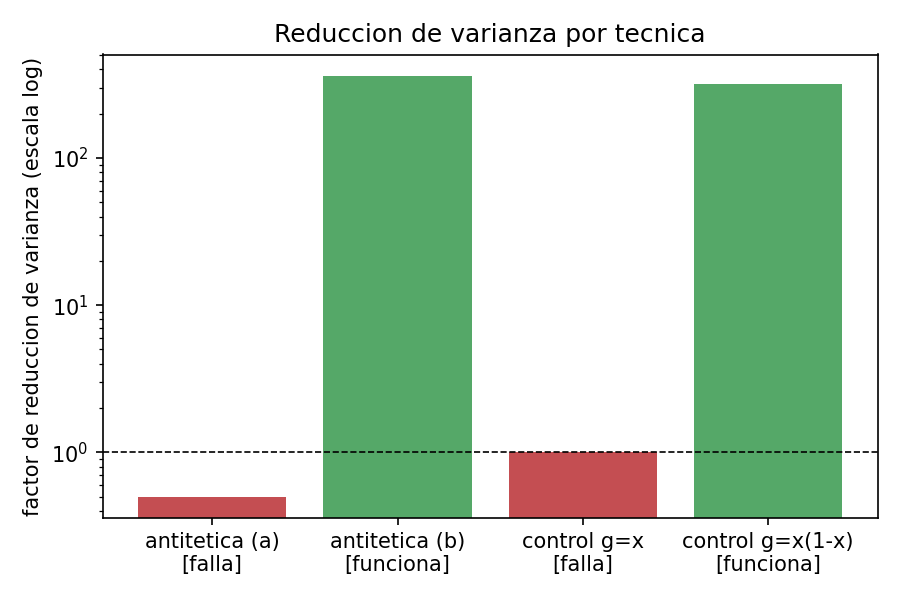
\includegraphics[width=0.6\textwidth]{figures/reduccion_varianza.png}
\caption{Factor de reducción de varianza logrado por cada técnica (escala logarítmica; la línea punteada marca el punto de equilibrio con Monte Carlo simple).}
\end{figure}

\subsection{¿Siempre ayuda, o depende del integrando?}

Los cuatro experimentos responden la pregunta de forma inequívoca: depende por completo del integrando y de qué tan bien elegida esté la técnica para su forma particular. Variables antitéticas solo funciona cuando $f$ tiene la simetría correcta (monotonía en el intervalo, como en (b)); aplicada a una función simétrica alrededor del punto medio del intervalo, como (a), el par antitético es redundante y el método empeora el desempeño respecto a Monte Carlo simple. Variables de control solo ayuda si se elige un control realmente correlacionado con el integrando: un control lineal simple no sirvió de nada para (a), mientras que un control con la forma correcta (una joroba simétrica) redujo la varianza en más de dos órdenes de magnitud. La lección práctica es que ninguna de estas técnicas es una mejora automática: hay que entender la forma del integrando antes de elegir cuál aplicar, y una elección descuidada puede incluso ser contraproducente.

\section{Cuando el generador arruina el resultado: el caso RANDU}
\label{sec:randu}

Se usó la implementación propia de RANDU para estimar por Monte Carlo la integral que da el enunciado, $\iiint_{[0,1]^3} \mathbf{1}[x^2+y^2+z^2\le 1]\,dV$, cuyo valor real es $\pi/6 \approx 0.523599$, agrupando el flujo de valores de RANDU en ternas consecutivas sin traslape $(u_{3i}, u_{3i+1}, u_{3i+2})$. Se repitió exactamente el mismo experimento con el Mersenne Twister propio, con $N=1{,}000{,}000$ ternas en ambos casos.

\begin{table}[H]
\centering
\begin{tabular}{lccc}
\toprule
Generador & Estimado & IC 95\% & Error absoluto \\
\midrule
RANDU & 0.523233 & (0.522254, 0.524212) & 0.000366 \\
Mersenne Twister & 0.522841 & (0.521862, 0.523820) & 0.000758 \\
\bottomrule
\end{tabular}
\caption{Estimación de $\pi/6$ con $N=1{,}000{,}000$ ternas, valor real $0.523599$.}
\end{table}

El resultado es, a primera vista, contraintuitivo: en esta corrida particular RANDU no solo no fue peor que Mersenne Twister, sino que su error absoluto resultó incluso menor. Esto no contradice lo que se documentó en la Sección \ref{sec:randu-generador}: la razón es que el volumen de una bola es una cantidad simétrica bajo rotaciones, y la falla geométrica de RANDU (que sus ternas caigan sobre unos 15 hiperplanos en vez de llenar el cubo) no necesariamente sesga el conteo de cuántas de esas ternas caen dentro de una esfera centrada en el origen, porque cada uno de esos planos todavía cruza la esfera y aporta puntos de ambos lados de su frontera. Dicho de otro modo: no toda cantidad calculada con Monte Carlo es igualmente sensible a la falta de independencia entre coordenadas consecutivas.

Para exhibir la falla de manera inequívoca hay que mirar la estructura de las ternas directamente, no un resumen numérico que puede resultar insensible a ella. Se calculó, para cada terna $(u_i,u_{i+1},u_{i+2})$, la distancia de $9u_i - 6u_{i+1} + u_{i+2}$ al entero más cercano (recordando de la Sección \ref{sec:randu-generador} que esta expresión debe ser exactamente un entero $k$ para RANDU, por construcción):

\begin{table}[H]
\centering
\begin{tabular}{lcc}
\toprule
Generador & Distancia media al entero más cercano & Distancia máxima \\
\midrule
RANDU & 0.0000000000 & 0.0000000000 \\
Mersenne Twister & 0.249992 & 0.499992 \\
\bottomrule
\end{tabular}
\caption{Distancia de $9u_i-6u_{i+1}+u_{i+2}$ al entero más cercano, sobre 100{,}000 ternas.}
\end{table}

La diferencia es absoluta: las $100{,}000$ ternas de RANDU caen \emph{exactamente} sobre esos hiperplanos, sin ninguna desviación más allá del error de redondeo de punto flotante, mientras que en Mersenne Twister la misma expresión se comporta como una variable continua genuina, con una distancia promedio al entero más cercano de $0.25$ (justo lo que se espera si la parte fraccionaria de esa combinación lineal fuera uniforme). Esta es la prueba espectral de la Sección \ref{sec:randu-generador}, pero convertida en un número: no es que RANDU tienda a caer cerca de esos planos, es que cae sobre ellos con precisión exacta, siempre. La moraleja de esta tarea es sencilla y la confirma tanto la Parte 1 como este experimento: un método de Monte Carlo nunca va a ser mejor que su fuente de aleatoriedad, aunque el daño que haga esa fuente defectuosa no siempre sea visible en la primera cantidad que uno decida calcular con ella. Por eso la prueba espectral —revisar la estructura geométrica del generador directamente, no solo el resultado final de una aplicación particular— es indispensable antes de confiar en cualquier PRNG para simulación.

\end{document}
